\chapter{Noisy phase retrieval: a brief survey of applications and methods} 	\label{Sec:phase_retrieval}


\section{Mathematical model}	\label{Subsec:phase_retrieval-math_model}



Phase retrieval is the problem of recovering a signal from magnitude-only observations with little or no knowledge of the signal phase.  Let $\bar{x}$ be a signal in $\bbR^n$ or $\bbC^n$ which as been observed with sensing (or sampling) vectors $a_i \in \bbC^m$, resulting in squared measurements $|\langle a_i, \bar{x} \rangle |^2 = \bar{b}_i \in \bbR$ for $i = 1, \ldots, m$.  Also assume the \textit{true observation} vector $\bar{b} = [\bar{b}_1, \ldots, \bar{b}_m]^T \in \bbR^m$ has been contaminated by possibly nontrivial noise $\eta = [\eta_1, \ldots, \eta_m]^T \in \bbR^m$, giving the observation vector $b = \bar{b} + \eta \in \bbR^m$.  Then we define the \textit{phase retrieval problem} as
\begin{equation} \label{Eqn:phase_retrieval}
\begin{array}{lll}
\textnormal{find}		&	x		\\
\st				&	|\langle a_i, x \rangle|^2 = b_i = \bar{b}_i + \eta_i	&	1 \leq i \leq m.
\end{array}
\end{equation}
If $\eta_i = 0$ for all $i$, then (\ref{Eqn:phase_retrieval}) is the noiseless phase retrieval problem (from \cite{Fienup82} and  \cite{DBLP:journals/tit/CandesLS15} among many others).  In this dissertation however, we are primarily concerned with nontrivial noise and will refer to (\ref{Eqn:phase_retrieval}) with $||\eta|| > 0$ as \textit{noisy phase retrieval}.  Additionally, we are concerned with noise $\eta$ which has a Gaussian distribution, as discussed in \cite{DBLP:journals/siamis/CandesESV13} and \cite{DBLP:journals/siamsc/FriedlanderM16}.


Each sensing vector $a_i \in \bbC^n$ is typically the conjugate of the $i$th row of the $n-$dimensional discrete Fourier transformation (DFT) matrix $F$ \cite[Chapter 11]{bracewell1986fourier}.  This gives the constraint $|Fx|^2 = b$ (where the square operator is applied element-wise).  Often the number of observations $m = nL$ is oversampled by a factor of $L$ to promote uniqueness of a signal solution and convergence of a given algorithm.  

The domain of the constraint in (\ref{Eqn:phase_retrieval}) is a high-dimensional torus, and thus phase retrieval is inherently nonconvex.  When deciding how to handle a particular phase retrieval problem, this  nonconvexity presents a unique challenge in terms of choosing an appropriate algorithm.  


In this chapter, we begin by discussing a few typical applications of phase retrieval and the experimental models used for our numerical testing.  
We then review several methods for noisy phase retrieval.  
These methods are split into three classes: alternating projection methods (Section \ref{Subsubsec:phase_retrieval-alternating_direction_methods}), structured optimization methods (Section \ref{Subsubsec:phase_retrieval-structured}) which rely on additional assumptions like sparsity of the signal $x$, and unstructured optimization methods (Section \ref{Subsubsec:phase_retrieval-unstructured}) which only require an observation vector $b$ and noise ratio $\epsilon_{\text{rel}} = ||\eta|| / ||b||$.  
This final class includes the PLGD model (\ref{Eqn:PhaseLift-GD}) which is central to this dissertation, and thus we provide greater detail for theoretical guarantees and numerical performance behavior.
Section \ref{Subsec:phase_retrieval-why_optimize_PLGD_model} closes this chapter with a justification for using the PLGD model (\ref{Eqn:PhaseLift-GD}) to handle noisy phase retrieval problems.
We see that the PLGD model is particularly well suited for developing a first-order optimization method.
Additionally, we demonstrate that one such first-order method for the PLGD model (Algorithm \ref{Alg:PGD} from Chapter \ref{Sec:PLGD_algo}) is generally more accurate and robust to noise and low oversampling than wflow, an alternative method discussed in Section \ref{Subsubsec:phase_retrieval-unstructured}.





\section{Applications and experimental models} 			\label{Subsec:phase_retrieval-applications}


Phase retrieval has a broad range of applications across the sciences, many of which fall into the general category of coherent diffraction imaging (CDI) \cite{miao1999extending}.  This section provides a brief overview of CDI and closes with a description of the phase retrieval experimental models used in this dissertation (as well as \cite{DBLP:journals/siamis/CandesESV13}, \cite{DBLP:journals/tit/CandesLS15}, \cite{DBLP:journals/siamsc/FriedlanderM16}).


More specific applications of phase retrieval can be found in astronomy \cite{fienup1987phase}, diffraction and array imaging \cite{bunk2007diffractive} \cite{chai2010array}, microscopy \cite{miao2008extending}, optics \cite{walther1963question}, and x-ray crystallography \cite{harrison1993phase}, \cite{millane1990phase} (for a recent benchmark set of crystallography problems, see \cite{elser2017benchmark}).  For a comprehensive introduction to optical phase retrieval and an overview of recent theory and methods, see the survey \cite{DBLP:journals/spm/ShechtmanECCMS15}.


CDI is a method for reconstructing $2$- or $3$-dimensional nano-structures (e.g., nanotubes, nanocrystals, proteins).  In this process, highly coherent waves (e.g., x-rays, electrons, photons) are projected at a given object.  The resulting diffraction creates a pattern of intensities which are measured with a detector, resulting in magnitude-only measurements.  Figure \ref{Fig:CDI} below depicts the CDI observation process.

\begin{figure}[H]
  \centering
    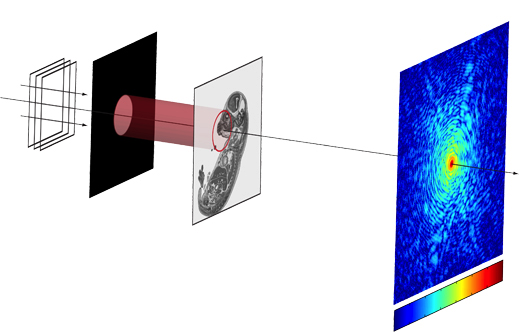
\includegraphics[width=0.75\textwidth]{phase_retrieval_depiction_mod.jpg}
   \caption{Depiction of coherent diffractive imaging.  Coherent waves (left) are projected at an image (center) which causes a diffraction pattern that is measured by a detector (right). Image from \cite{Guizar-Sicairos}.}
   \label{Fig:CDI}
\end{figure}

Because CDI does not involve optical lenses, there is no optical aberration (blurring or distorting).  Instead, the resolution depends on the limits of diffraction and dose.  Many efficient methods exist for handling low-noise phase retrieval (see Section \ref{Subsubsec:phase_retrieval-alternating_direction_methods} for an overview of a few common methods).  However, due to the nonconvexity of the constraints in (\ref{Eqn:phase_retrieval}), these low-noise methods are often likely to diverge or converge to a suboptimal local minimum if there is modest noise or an insufficient number of observations.  Thus accurate CDI typically requires minimal noise and multiple observations to recover a high-resolution solution.




When developing an experimental model, there are many methods for increasing the number of observations of a signal.  Some options include rotating the position of the object, using a spatial light modulator to defocus the observations, and inserting phase plates, or \textit{masks}, in line with the waves (see the survey \cite{duadi2011digital} for a discussion of these methods).  Our experimental models use the same masking method described in \cite[Section 2]{DBLP:journals/siamis/CandesESV13}, \cite[Sections 4.2, 4.3]{DBLP:journals/tit/CandesLS15}, and \cite[Section 5.1]{DBLP:journals/siamsc/FriedlanderM16} (see Section \ref{Subsubsec:phase_retrieval-unstructured} for an overview of these papers).  This masking method involves placing a phase plate with a known structure oriented normal to the projected waves.  The phase plate can be placed on either side of the object; in our experiments, the plate lies between the object and the detector.  The mask is then shifted and multiple observations are collected.




Mathematically, the application of a phase plate to the phase problem (\ref{Eqn:phase_retrieval}) is equivalent to replacing the sensing operator $|Fx|^2$ with $|FC_jx|^2$, where the matrices $C_j \in \mathbb{C}^{n \times n}$ are diagonal with standard Gaussian distribution entries $C_j(i,i) \sim \caN(0, 1)$, representing the diffraction patterns of the shifted phase plate.  This gives the observation constraint

\begin{equation}		\label{Eqn:FCx}
	\begin{vmatrix}
		FC_1x \\ \vdots \\ FC_Lx
	\end{vmatrix}^2
	= b.
\end{equation}

In certain cases only a limited number of observations can be collected.  For instance, in x-ray imaging, overexposure of the incident waves to the object (living tissue) can be dangerous.  Thus the number of observations $L$ may be relatively small compare to the signal size $n$, making signal recovery difficult for nonconvex methods.





In this dissertation, our experimental phase retrieval models are generating using the method established in \cite{DBLP:journals/tit/CandesLS15} and extended in \cite{DBLP:journals/siamsc/FriedlanderM16}.  
We begin with a signal $x$ which is either a vectorized image or a randomly generated vector with coordinates having complex standard Gaussian distribution $x_i \sim \caN(0, 1)$.
Next, we generate $j = 1, 2, \ldots,  L$ diagonal mask matrices $C_j \in \mathbb{C}^{n \times n}$ with diagonal entries $C_j(i,i) \sim \caN(0, 1)$.
We then compute the product (\ref{Eqn:FCx}) to obtain the true observation vector $\bar{b}$.
For noiseless phase retrieval, we set the observation vector to $b = \bar{b}$.
If the phase retrieval problem requires a nonzero noise term $\eta$, we add $\eta$ to the true observation to obtain the observation vector $b = \bar{b} + \eta$.
Figure \ref{Fig:parrot_signal_iterates} below depicts the primary test image used in this dissertation.
Here, an original image of size $128 \times 128$ is used to generate a noisy phase retrieval problem, and we see a few particular iterates returned by the method considered in this dissertation (Algorithm \ref{Alg:PGD} in Section \ref{Subsec:PLGD_algo-algo}).  
For a complete explanation of our method for creating noisy phase retrieval problems, see Section \ref{Subsec:PLGD_term_crit-NOISY_MODELS_AND_RESIDUALS}.

\begin{figure}[H]
\centering
\hbox{\hspace{-2.3cm} 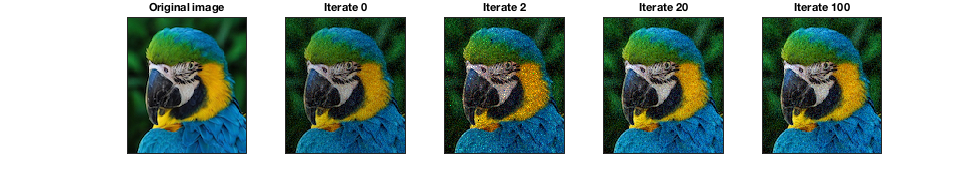
\includegraphics[scale=0.55]{parrot_signal_iterates} }
\caption{Results from a first-order method (Algorithm \ref{Alg:PGD} in Section \ref{Subsec:PLGD_algo-algo}) applied to a noisy phase retrieval problem (\ref{Eqn:phase_retrieval}) with oversampling rate $L = m/n=8$ and noise ratio $\epsilon_\text{rel} = ||\eta|| / ||b|| = 0.30$.}
\label{Fig:parrot_signal_iterates}
\end{figure}
% experiments.figure.noisyimage_signal_relerr_various_saga_iterates




\section{Survey of noisy phase retrieval methods}  	\label{Subsec:phase_retrieval-survey_of_methods}

Due to the variety of phase retrieval applications and the difficulty of solving the phase retrieval problem (\ref{Eqn:phase_retrieval}), a wide range of phase retrieval methods have been developed for both noisy and noiseless phase retrieval.  This section provides a review of methods for noisy phase retrieval (\ref{Eqn:phase_retrieval} with $||\eta|| > 0$) which we separate into three classes: alternating projection methods (Section \ref{Subsubsec:phase_retrieval-alternating_direction_methods}), structured optimization methods (Section \ref{Subsubsec:phase_retrieval-structured}), and unstructured optimization methods (Section \ref{Subsubsec:phase_retrieval-unstructured}).  These three classes were chosen to mirror the historical progression of methods (as the alternating projection methods preceded the others by a few decades) and emphasize the uniqueness of the three unstructured methods discussed in Section \ref{Subsubsec:phase_retrieval-unstructured}.  For a recent survey of noiseless phase retrieval methods, see \cite{DBLP:journals/corr/JaganathanEH15a}.








\subsection{Alternating projection methods}		\label{Subsubsec:phase_retrieval-alternating_direction_methods}



We begin by discussing alternating projection methods for phase retrieval.  These methods were established in the 1970s and 1980s as the first strategy for solving (\ref{Eqn:phase_retrieval}) and rely on prior information about the signal, such as support constraints or positivity.  Originally referred to as \textit{error reduction algorithms}, these methods were later identified as nonconvex alternating projection methods \cite{LeviS84}.  Each of these methods relies on projecting an iterate between the \textit{object domain} (or time domain) in which we seek the desired signal $\bar{x}$, and the \textit{frequency domain} in which we have the observation $b$.  

We begin with two common alternating projection methods: the Gershberg-Saxton (GS) algorithm \cite{GS72} and the hybrid input-output (HIO) algorithm \cite{Fienup82}, a variant of the GS algorithm which is still commonly used in practice.  
We then discuss recent alternating projection methods for noisy phase retrieval (oversampling smoothness (OSS) \cite{rodriguez2013oversampling}, error reduction (ER-) HIO and noise robust (NR-) HIO \cite{martin2012noise}).
Note that these these alternating projection algorithms are usually not effective for noisy phase retrieval and typically require additional prior information.
Nevertheless, the discussion in this section will be relevant in Section \ref{Subsubsec:phase_retrieval-unstructured} when we discuss the wflow algorithm \cite{DBLP:journals/tit/CandesLS15}, which can also be viewed as an alternating projection method.  





Developed in 1972, the GS algorithm was the first alternating projection method for phase retrieval and serves as an algorithmic foundation which later alternating projection methods would modify to improve the likelihood of convergence.  
Given the phase retrieval problem (\ref{Eqn:phase_retrieval}) with no oversampling (i.e., $L=1$) and knowledge of the signal magnitude $c \in \bbR^n_+$ (i.e., $c_i = |\bar{x}_i|^2$ for all $i$), we may attempt to solve (\ref{Eqn:phase_retrieval}) with Algorithm \ref{Alg:GS}.

\begin{algorithm}[H]
\caption{Gershberg-Saxton (GS) algorithm}	\label{Alg:GS}

\begin{algorithmic}[1]
	\Statex 	\textbf{Input:} Observation vector $b \in \bbR^n_+$, signal measurement vector $c \in \bbR^n_+$, DFT matrix $F \in \bbC^{n \times n}$.
	\Statex 	\textbf{Output:} Approximate solution signal $x \in \bbC^n$.
	\State 		\textit{Initialize:} Choose a random signal $x_0 \in \bbC^n$, compute DFT $y_0 = F x_0$, set $res=|y_0|^2 - b$, $k = 0$.
	\While {$||res|| > \textnormal{tol}$}
		\State 	Compute DFT of $x_k$ and residual: $y_{k+1} = F x_k$, $res = |y_{k+1}|^2 - b$.
		\State	Impose observation magnitude constraints: $[y_{k+1}]_i = \frac{[y_{k+1}]_i}{|[y_{k+1}]_i|} \sqrt{b_i}$ for all $i = 1, \ldots, n$.
		\State	Compute inverse DFT of $y_{k+1}$: $x_{k+1} = F^{-1} y_{k+1}$.
		\State	Impose signal magnitude constraints: $[x_{k+1}]_i = \frac{[x_{k+1}]_i}{|[x_{k+1}]_i|} \sqrt{c_i}$ for all $i = 1, \ldots, n$.
		\State	$k = k + 1$.
	\EndWhile	\\
	\textit{Return:} $x = x_k$.
\end{algorithmic}
\end{algorithm}

During an iteration of the GS algorithm, knowledge of the signal and observation magnitudes, as well as any additional information, is applied when the iterate reaches that respective domain (steps 6 and 4, respectively).  While the GS algorithm is notable as the first algorithmic phase retrieval method, this algorithm is also very likely to converge to a local rather than global minimum \cite{DBLP:journals/corr/JaganathanEH15a}.




In \cite{Fienup82},  Fienup interpreted the GS algorithm as a nonlinear feedback control system (Figure \ref{Fig:nonlinear_feedback_control_system}), where the \textit{System} component corresponds to the map $\widetilde{P}_\textnormal{freq} = F^{-1} P_\textnormal{freq} F$ (combining steps 3-5 of the GS algorithm, where $P_\textnormal{freq}$ is projection onto the frequency constraints in step 4).  Since the GS algorithm interprets phase retrieval as an error-reduction problem, the system output $\widetilde{P}_\textnormal{freq}(x_k)$ is viewed as the current candidate for the desired signal $\bar{x}$, and the signal magnitude constraints (GS algorithm, step 6) are imposed to arrive at a new input $x_{k+1}$ which is considered the current approximation to the solution signal.  By viewing phase retrieval as a nonlinear feedback problem, the input $x_k$ is no longer treated as a signal approximation, and instead serves as feedback information for the system.  Thus $x_k$ need not satisfy the signal magnitude constraints.


\begin{figure}[H]
\centering

\tikzstyle{block} = [rectangle, draw, fill=white!20,
    text width=5em, text centered, rounded corners, minimum height=4em]
\tikzstyle{line} = [draw, -latex']

\begin{tikzpicture}[align=center, node distance = 5cm, auto]
    % Place nodes
    \node [block] (system) {System};
    \node [block, right of=system] (sensor) {Sensor};
	\node [block, left of=system] (controller) {Controller};
	\draw[<-] (controller) -- +(-25mm,0) node [left] (reference) {} node [below] {reference};
	\draw[->] (sensor) -- +(25mm,0) node [right] (solution) {} node [below] {solution};

	% Draw edges
	\path [->] (system) edge node [below] {output}
										    node [above] {$\widetilde{P}_\textnormal{freq}(x_k)$} (sensor);
	\path [line] (sensor) -- ++  (0,-3cm) -| (controller);
	\path [->] (controller) edge node [below] {input} node [above] {$x_k$} (system);
\end{tikzpicture}

\caption{Phase retrieval as a nonlinear feedback control system} \label{Fig:nonlinear_feedback_control_system}
\end{figure}


Fienup observed that a small change in the input will result in an output that is approximately a constant $\alpha$ times the change in the input, that is
\begin{equation} 		\label{Eqn:HIO_linear_appx}
	\widetilde{P}_\textnormal{freq}(x + \Delta x) - \widetilde{P}_\textnormal{freq}(x) \approx \alpha \Delta x.
\end{equation}
To force a change of $\Delta x$ in the output $\widetilde{P}_\textnormal{freq}(x)$, the input would logically be changed by $\beta \Delta x$, where $\beta = 1/\alpha$ from (\ref{Eqn:HIO_linear_appx}).  This observation led Fienup to identify three new potential strategies for selecting an update (the \textit{Controller} in Figure \ref{Fig:nonlinear_feedback_control_system}).  The most successful of these methods is the HIO algorithm, which has the following index-wise update replacing step 6 in the GS algorithm:
\begin{equation} 		\label{Eqn:HIO_step_6}
[x_{k+1}]_i =
	\begin{cases}
		[\widetilde{P}_\textnormal{freq}(x_k)]_i	&	i \notin \caV		\\
		[x_k]_i - \beta [\widetilde{P}_\textnormal{freq}(x_k)]_i			&	 i \in \caV,
	\end{cases}
\end{equation}
where $\caV$ is the set of indices in which the update violates the object domain constraints.  This simple corrective step (\ref{Eqn:HIO_step_6}) which HIO applies to the object domain makes the resulting algorithm much more likely than the GS algorithm to recover a signal from a low-noise observation \cite{DBLP:journals/corr/JaganathanEH15a}.   Nevertheless, HIO still has a tendency to converge to local minima and is not robust to noise.  In practice, the user will often select a large number of random initial iterates to initialize HIO and select the best resulting signal.




Recent developments in alternating projection methods for phase retrieval have focused on handling noisy observations.  In \cite{rodriguez2013oversampling}, the authors modify the GS algorithm by taking the HIO update (\ref{Eqn:HIO_step_6}) and performing a Gaussian smoothing step in the frequency domain on the indices (pixels) violating the support constraint.  Their oversampling smoothness (OSS) algorithm takes the update $x_{k+1}$ from HIO step 6 and applies the additional update:
\begin{equation}
[x_{k+1}]_i =
	\begin{cases}
		[x_{k+1}]_i		&	i \notin \caV		\\
		\left[ F^{ -1} \left[ F ( x_{k+1}) \ .* \bar{w}(j, \alpha) \right]  \right]_i	&	 i \in \caV,
	\end{cases}
\end{equation}
where $j = 1, \ldots, N$ is the Fourier index, $.*$ is pointwise multiplication, and $\bar{w}(j, \alpha)$ is a normalized Gaussian function
\[
\bar{w}(j, \alpha) = e^ {- \frac{1}{2} \left(\frac{j}{\alpha} \right)^2}.
\]
As $\alpha \rightarrow \infty$, the original HIO algorithm is recovered.  The authors select $\alpha$ heuristically, with early $\alpha = \caO(N)$ and later $\alpha = \caO(1/N)$, causing the OSS algorithm to behave similarly to HIO during early iterations while damping high frequency violations in later iterations.  Their experiments \cite[Section 3]{rodriguez2013oversampling} apply Poisson noise with noise levels ranging from 0.05 to 0.25 (and measured in the $1$-norm, but approximately equivalent to our definition $\epsilon_\textnormal{rel} = ||\eta|| / ||b||$).  The results suggest that the accuracy and consistency of the OSS algorithm is superior to HIO and two HIO variants: ER-HIO and NR-HIO of \cite{martin2012noise}.  



While these HIO-type methods are computationally efficient and still commonly used in practice \cite{DBLP:journals/corr/JaganathanEH15a}, they also require special parameter tuning (e.g., $\beta$ in HIO and $\alpha$, $\beta$ in OSS) and prior information about the desired signal.  Additionally, none of these methods are wholly robust to noise or guaranteed to converge, and require large batches of random initializations in practice to generate an adequate solution.  To overcome these deficiencies, recent phase retrieval methods have largely avoided the alternating projection framework, instead casting (\ref{Eqn:phase_retrieval}) as a structured optimization problem.





\subsection{Structured optimization methods}  	\label{Subsubsec:phase_retrieval-structured}


Next we discuss structured optimization methods for noisy phase retrieval.  In the past decade, a wide range of methods have been crafted to take advantage of the structure of particular phase retrieval problems.  The survey in this section highlights typical methods, their applications, and theoretical guarantees for exact recovery or error bounds.  


The methods in this section are grouped in terms of the structural property each seeks to exploit.  
The \textit{compressive phase retrieval} methods assume sparsity in the signal $x$, and include \cite{DBLP:journals/corr/abs-1104-4406}, the GrEedy Sparse PhAse Retrieval (GESPAR) method \cite{shechtman2014gespar}, and thresholded wflow  \cite{cai2016optimal}.
The \textit{robust phase retrieval} methods assume sparsity in either the observation $b$ \cite{katkovnik2017phase} or the noise $\eta$ \cite{jiang2017robust}.
The \textit{supervised phase retrieval} methods require an approximate solution signal $\hat{x}$ for initialization, and include \cite{goldstein2018phasemax} and \cite{bahmani2016phase}.



The authors of \cite{DBLP:journals/corr/abs-1211-0872} consider the theoretical recovery guarantees for compressive phase retrieval.
They prove signal uniqueness and stable recovery (a stronger property than invertibility) for a variety of sparsity assumptions.  
For instance, if the signal $x$ is $k$-sparse and observation $b$ is noiseless, then $\caO(k \log(n/k))$ observations are necessary for signal uniqueness.  
If $x$ is $k$-sparse and $b$ is noisy, then $\caO(k \log(n/k) \log(k))$ observations are necessary to guarantee stable recovery (which gives $\caO(n \log(n))$ observations if $x$ dense).


Many methods have been considered for handling compressive phase retrieval.  In \cite{DBLP:journals/corr/abs-1104-4406}, the authors consider sparse signals with noisy observations and proceed by lifting the signal and sensing vectors (for details on lifting and the PhaseLift model, see Section \ref{Subsubsec:phase_retrieval-unstructured}).  They construct a rank minimization problem similar to the PhaseLift rank minimization model, but with an additional mixed $1,2$-norm constraint
\[
	\sum\limits_{\substack{i = 1}}^{\substack{n}}
	\left( 	\sum\limits_{\substack{j = 1}}^{\substack{n}}  X_{i, j}^2
	\right)^{1/2}
	\leq \zeta
\]
which promotes row-sparsity of the lifted solution matrix $X$.  The resulting algorithm also includes a thresholding step on the spectrum of $X$ to enforce low-rankness in the solution.   The authors provide comparative numerical results indicating the addition of this constraint/thresholding strategy in their optimization method decreases reconstruction error as the noise ratio increases.  However, the overall model is nonconvex, the iterations are expensive (each requiring the inversion of a lifted matrix), and no theory is provided to guarantee convergence or signal recovery quality.


The GESPAR method of \cite{shechtman2014gespar} assumes $x$ is $k$-sparse and $b$ is noisy, and constructs an algorithm which maintains an active set $S$ of indices which converges to the appropriate $k$-sized set of active indices in the solution signal.  This local search method does not require matrix lifting, making it efficient for large-scale phase retrieval.  Numerical results \cite[Section 5]{shechtman2014gespar} indicate that as sparsity increases, GESPAR has a higher recovery probability than PhaseLift and a sparse variant of HIO.

A thresholded version of the wflow algorithm (see Section \ref{Subsubsec:phase_retrieval-unstructured} for wflow) is considered in \cite{cai2016optimal}.  Under the assumption that $x$ is sparse and $b$ is noisy, the authors develop a thresholded gradient descent algorithm by adding $\tau ||x||_1$ to the wflow objective function
\begin{equation}
\begin{array}{ll}
	\min\limits_{\substack{x}}
		&	\frac{1}{2m} \sum\limits_{\substack{i=1}}^{\substack{m}} \left( |a_i^*x|^2 - b_i \right)^2
			+ \tau ||x||_1.
\end{array}
\end{equation}
The authors show that this phase retrieval analog to the basis pursuit denoising model \cite{chen2001atomic} has the minimax optimal rate of convergence, $\caO (k \log(n) / m)$, for the proper choice of $\tau$.

Another recent method for compressive phase retrieval considers unstructured noise $\eta$ in the observation, and interprets the recovery of a $k$-sparse signal $x$ as a covariance maximization problem between the observations $b_i$ and the sensing values $|a_i^*x|^2$ over the appropriate $k$-dimensional subspace \cite{zhang2017fast}.  The authors show that only $\caO(k)$ measurements are required for their algorithm to converge within $\epsilon$ error in a runtime of $\caO(nk \log(1/ \epsilon))$ iterations.




Other recent papers consider robust phase retrieval, where we find sparsity in the observation space rather than the signal space.  In one case, the paper \cite{jiang2017robust} assumes the noise $\eta$ is sparse.  Whereas the minimization of the $2$-norm is optimal for fitting against Gaussian noise, the $1$-norm is more robust for distributions with heavier tails.  Thus the authors suggests minimizing the objective function $||\caA(xx^*) - b||_1$ and develop an alternating direction method of multipliers (ADMM) algorithm.  Their work provides numerical results which demonstrate that this method achieves better accuracy than the wflow algorithm when recovering from an observation with Gaussian noise and 10\% outliers.

In contrast, the authors of \cite{katkovnik2017phase} consider phase retrieval when the observation vector $b$ is itself sparse and noisy.  Their algorithm is a HIO-type algorithm, with noise suppression in the frequency domain and phase/amplitude filtering in the object domain.  Numerical results show this algorithm achieves better accuracy under the given sparsity assumptions than wflow and a filtered version of the GS algorithm.





Rather than assuming sparsity of the signal or observations, the authors of \cite{goldstein2018phasemax} and \cite{bahmani2016phase} assume the existence of an approximation $\hat{x}$ to the solution signal $\bar{x}$.  In this supervised phase retrieval paradigm, the authors define the PhaseMax model
\begin{equation} 			\label{Eqn:PhaseMax}
\begin{array}{lll}
	\max\limits_x	&	\Re \langle \hat{x}, x \rangle 		\\
	\st 			&	| \langle a_i, x \rangle |^2 \leq b_i, 	&	i = 1, \ldots, m,
\end{array}
\end{equation} 
where $\Re(\cdot)$ maps a complex number to its real component.  The PhaseMax model (\ref{Eqn:PhaseMax}) has the benefits of being convex without requiring signal lifting.  The dual to this problem is the widely-studied basis pursuit problem which has several efficient solution techniques \cite{chen2001atomic}, \cite{candes2006stable}.  The authors of \cite{goldstein2018phasemax} prove that the probability of exact recovery is dependent on the angle between $\bar{x}$ and $\hat{x}$.
Their numerical results demonstrate that this probability quickly approaches $1$ as oversampling increases.




\subsection{Unstructured optimization methods}	 	\label{Subsubsec:phase_retrieval-unstructured}


The final class of methods we examine are unstructured optimization methods.  Unlike the methods discussed in Section \ref{Subsubsec:phase_retrieval-structured}, these methods place no assumptions on the signal $x$, the sensing vectors $a_i$, or the observation $b = \bar{b} + \eta$ other than knowledge of the noise ratio $\epsilon_\rel = ||\eta|| / ||b||$.

This section begins with an explanation of matrix lifting for the signal and sensing vectors.  Next we discuss the PhaseLift model \cite{DBLP:journals/siamis/CandesESV13} and the wflow algorithm \cite{DBLP:journals/tit/CandesLS15}.   Theoretical and numerical results are included to highlight the effectiveness and robustness of these models and methods (for complete theoretical results, see \cite{DBLP:journals/tit/CandesLS15},  \cite{sun2016geometric} for wflow and \cite{candes2014solving}, \cite{candes2013phaselift} for PhaseLift).  This discussion of PhaseLift and wflow leads us to the PhaseLift gauge dual model \cite{DBLP:journals/siamsc/FriedlanderM16}, another unstructured optimization model which is the subject of Chapter \ref{Sec:PLGD}.






The PhaseLift model was first introduced in \cite{DBLP:journals/siamis/CandesESV13}, with additional theoretical results established in \cite{candes2013phaselift}.  This model is based on the concept of matrix lifting.  First we define the linear operator $\caA$ which allows us to lift the nonlinear phase retrieval observation constraint from (\ref{Eqn:phase_retrieval}) into a higher-dimensional linear constraint.  If we lift the $n$-dimensional signal $x$ and sensing vectors $a_i$ into rank-one Hermitian matrices $X = xx^*, A_i = a_ia_i^* \in \caH^n$, then the sensing operator $\caA$ is defined coordinate-wise to satisfy $[\caA (X)]_i = \langle A_i, X \rangle = \tr( a_i a_i^* xx^* )= | \langle a_i, x \rangle |^2$.  Thus $\caA: \caH^n \rightarrow \bbR^m$ and its adjoint $\caA^* : \bbR^m \rightarrow \caH^n$ are defined as
\begin{equation} 			\label{Eqn:A_definition}
\begin{array}{lcr}
\caA(xx^*)
	:= \begin{bmatrix} \langle a_1 a_1^*, xx^* \rangle \\ \vdots \\ \langle a_m a_m^*, xx^* \rangle \end{bmatrix}
		
	& 	\text{and}
		&	\caA^*y
			  := \sum\limits_{\substack{i = 1}}^{\substack{m}} y_ia_ia_i^*.
\end{array}
\end{equation}
In particular, if the experimental model is the one discussed in Section \ref{Subsec:phase_retrieval-applications} then we have
\begin{equation} 			\label{Eqn:A_definition_with_masks}
\begin{array}{l}
\caA(xx^*)
		= \begin{vmatrix}
				FC_1x \\ \vdots \\ FC_Lx
			\end{vmatrix}^2
			= \textnormal{diag}\begin{bmatrix}
			\begin{pmatrix}
			FC_1 \\ \vdots \\ FC_L
			\end{pmatrix}
		 	(xx^*)
	 		\begin{pmatrix}
			FC_1 \\ \vdots \\ FC_L
		 	\end{pmatrix}^*
		\end{bmatrix},
									\\
									\\
\caA^*y
			  =\sum\limits_{\substack{j=1}}^{\substack{L}}
					[FC_j]^* \textnormal{Diag}(y_j) F C_j.
\end{array}
\end{equation}






The lifted rank-one matrix $X = xx^* \in \caH^n$ and sensing operator $\caA$ are then used to lift the nonlinear phase retrieval constraints $| \langle a_i, x \rangle | ^2 = b_i$ for $i = 1, \ldots, m$ into the linear constraint $\caA(X) = b$.  Thus (\ref{Eqn:phase_retrieval}) is equivalent to the left-most problem in the sequence of problems
\begin{equation} 		\label{Eqn:PhaseLift_rank_model}
\begin{array}{ll}
		\textnormal{find}
		&	x
			\\
		\st
		& 	\caA (xx^*) = b
\end{array}
\iff
\begin{array}{ll}
		\textnormal{find}
		&	X
			\\
		\st
		& 	\caA (X) = b
			\\
		&	X \succeq 0
			\\
		&	\textnormal{rank}(X) = 1
\end{array}
\iff
\begin{array}{ll}
		\min\limits_{\substack{X \in \caH^n}}
		&	\textnormal{rank}(X)
			\\
		\st
		& 	\caA (X) = b
			\\
		&	X \succeq 0.
\end{array}
\end{equation}
If a rank-one solution  $X = xx^*$ exists then this matrix satisfies the lifted model in the middle of (\ref{Eqn:PhaseLift_rank_model}), and the left implication holds.  Likewise, the rank minimization model at right in (\ref{Eqn:PhaseLift_rank_model}) will have a rank-one solution, and the right implication holds.  





The resulting rank minimization problem at right of (\ref{Eqn:PhaseLift_rank_model}) is NP hard, as it includes the cardinality minimization problem as a special case (see \cite{natarajan1995sparse} or  \cite{recht2010guaranteed}).  Thus the next step is to relax the discrete, nonconvex objective function $\textnormal{rank}(X)$.  To generalize the right-most model in (\ref{Eqn:PhaseLift_rank_model}) for noisy phase retrieval, a norm bound is also applied to the sensing constraint.  This gives the semidefinite program which defines the PhaseLift model \cite{DBLP:journals/siamis/CandesESV13}, \cite{candes2013phaselift}
\begin{equation} \label{Eqn:PhaseLift}
\begin{array}{lll}
	&	\min\limits_{\substack{X \in \caH^n}}
		&	||X||_1 = \sum\limits_{\substack{i=1}}^{\substack{n}} \sigma_i(X)
			\\
\textnormal{(PhaseLift)}
	&	\st
		& 	||\caA (X) - b||_2 \leq \epsilon
			\\

	&
		&	X \succeq 0.

\end{array}
\end{equation}
Here the objective function $||X||_1$ refers to the Schatten $p$-norm (which is expressed as $\sum_{i=1}^n \sigma_i(X)$, $\tr(X)$, or $\langle I, X \rangle$ in various literature).  Also, the term $\epsilon = ||\eta||$ measures the total noise, whereas $\epsilon_\rel = ||\eta|| / ||b||$ discussed in Section \ref{Subsec:phase_retrieval-applications} measures the noise ratio (or relative noise).  We choose the Schatten $p$-norm to highlight the fact that (\ref{Eqn:PhaseLift}) is the semidefinite analog to the celebrated  basis pursuit denoising problem \cite{chen2001atomic}, \cite{candes2006stable},

\begin{equation}  			\label{Eqn:basis_pursuit}
\begin{array}{lll}
	&	\min\limits_{\substack{x}}
		&	||x||_1
			\\
	&	\st
		&	||Ax-b||_2 \leq \epsilon,
\end{array}
\end{equation}
where minimizing $||x||_1$ serves as a convex relaxation to minimizing the discrete, nonconvex function $||x||_0 = \textnormal{nnz}(x)$.



The next two theorems quantify the relaxation of the PhaseLift model (\ref{Eqn:PhaseLift}) from the phase retrieval model (\ref{Eqn:phase_retrieval}), establishing exact and approximate recovery guarantees for the PhaseLift model \cite{candes2014solving}, \cite{candes2013phaselift}.  Theorem \ref{Thm:PhaseLift_exact} applies to the noiseless case (where $\epsilon = 0$ in the PhaseLift model), establishing a probability of equivalence between (\ref{Eqn:phase_retrieval}) and (\ref{Eqn:PhaseLift}).  


\begin{theorem}  \label{Thm:PhaseLift_exact}
Consider an arbitrary signal $\bar{x}$ in $\bbR^n$ or $\bbC^n$ and assume the sensing vectors $a_i$ are independent, uniformly distributed on the unit sphere of $\bbR^n$ or $\bbC^n$.  Suppose that the number of measurements obeys $m \geq c_0 n$, where $c_0$ is a sufficiently large constant. Then in both the real and complex cases, the solution to (\ref{Eqn:PhaseLift}) is exact with high probability in the sense that the noiseless PhaseLift problem (i.e., (\ref{Eqn:PhaseLift}) with $\epsilon = 0$) has a unique solution obeying
\[
X = \bar{x}\bar{x}^*.
\]
This holds with probability at least $1 - \caO(e^{-\gamma m})$, where $\gamma$ is a positive absolute constant.
\end{theorem}
\begin{proof}
See \cite[Section 2]{candes2014solving}.
\end{proof}




The assumptions of Theorem \ref{Thm:PhaseLift_exact} are met by the experimental models used in \cite{DBLP:journals/siamis/CandesESV13}, \cite{candes2013phaselift}, \cite{DBLP:journals/siamsc/FriedlanderM16}, and this dissertation (see Section \ref{Subsec:phase_retrieval-applications}, where the masks $C_i \in \bbC^{n \times n}$ from (\ref{Eqn:FCx}) have diagonal entries chosen with Gaussian distribution).  Thus, if $L$ is the oversampling rate (i.e., $m = nL$) then Theorem \ref{Thm:PhaseLift_exact} shows that only $L = \caO(1)$ masks are required to guarantee exact signal recover (up to global phase) with high probability.




Theorem \ref{Thm:PhaseLift_approx} applies to the  noisy phase retrieval case ($\epsilon > 0$), where there is no guarantee that the PhaseLift (\ref{Eqn:PhaseLift}) solution matrix $X$ is low rank.  Thus the solution signal $x$ is set to an appropriate rescaling of the eigenvector $v_1$ corresponding to the algebraically largest eigenvalue $\lambda_1 = \lambda_1 (X)$, giving
\begin{equation}  			\label{Eqn:PhaseLift_solution_signal}
x = \sqrt{\lambda_1}v_1.
\end{equation}

\begin{theorem}  \label{Thm:PhaseLift_approx}
Consider an arbitrary signal $\bar{x}$ in $\bbR^n$ or $\bbC^n$ and assume the sensing vectors $a_i$ are independent, uniformly distributed on the unit sphere of $\bbR^n$ or $\bbC^n$.  Also suppose that the number of measurements obeys $m \geq C_0 n \log n $, where $C_0$ is a sufficiently large constant.  Then the PhaseLift (\ref{Eqn:PhaseLift}) solution $X$ obeys
\begin{equation}				\label{Eqn:Thm_PhaseLift_approx_X}
||X - \bar{x}\bar{x}^*||_F \leq C_0 \epsilon,
\end{equation}
for some positive constant $C_0$.  Additionally, we have
\begin{equation}		\label{Eqn:Thm_PhaseLift_approx_x}
||x - e^{i \theta}\bar{x}||_2 \leq C_0 \min(||\bar{x}||_2, \epsilon / ||\bar{x}||_2),
\end{equation}
where $x$ is defined as in (\ref{Eqn:PhaseLift_solution_signal}) and $\theta \in [0, 2\pi]$.
Both of these estimates hold with probability at least $1 - \caO(e^{-\gamma \frac{m}{n}})$, where $\gamma$ is a positive absolute constant.
\end{theorem}
\begin{proof}
See \cite[Section 6]{candes2013phaselift}.
\end{proof}


The strength of the PhaseLift model lies in its convexity and generality (no signal or observation assumptions are necessary).  Yet the weakness is the difficulty in optimizing the objective function $||X||_1$, as its evaluation requires a partial SVD.




Like the PhaseLift method, the recent Wirtinger flow (wflow) algorithm \cite{DBLP:journals/tit/CandesLS15} also seeks to solve the phase retrieval problem (\ref{Eqn:phase_retrieval}) without any assumptions on the structure or sparsity of the signal or observation.  However, unlike the PhaseLift model, the wflow model does not involve matrix lifting and instead frames (\ref{Eqn:phase_retrieval}) as the least-squares problem
\begin{equation} 				\label{Eqn:wflow_least-squares}
\begin{array}{ll}
	\min\limits_{\substack{x}}
		&	\frac{1}{2m} \sum\limits_{\substack{i=1}}^{\substack{m}} \left( |a_i^*x|^2 - b_i \right)^2
			= \frac{1}{2m} || \caA(xx^*) - b||^2.
\end{array}
\end{equation}


While this model is nonconvex, the authors of \cite{DBLP:journals/tit/CandesLS15} develop an efficient gradient descent-like method which has a provable guarantee for exact recovery when initialized appropriately.  Initialization of the wflow algorithm involves a rescaling of the eigenvector $v_1$ corresponding to the algebraically largest eigenvalue of the matrix $\caA^*b$, which is itself the sum of the outer products of the measurement vectors, scaled with the observation magnitudes
\begin{equation}			\label{Eqn:wflow_initialization}
\caA^*b := \sum\limits_{\substack{i=1}}^{\substack{m}}b_i a_i a_i^*.
\end{equation}


The authors motivate this choice of intialization by noting that if the sensing vectors $a_i$ are i.i.d. with standard Gaussian distribution, and $||\bar{x}|| = 1$, then the expected value of the outer product sum $\caA^*b$ will be
\begin{equation} 		\label{Eqn:wflow_expected_value}
\bbE \left[ \frac{1}{m}\caA^* b \right] = I + 2\bar{x}\bar{x}^*.
\end{equation}
Thus for large $m$, (\ref{Eqn:wflow_initialization}) has a high probability of returning a vector $v_1$ closely aligned with the solution $\bar{x}$. Intuitively, this initialization can also be seen as maximizing $\langle \caA(vv^*), b \rangle	= \langle v v^*, \caA^* b \rangle = \langle v, [\caA^* b] v \rangle$.  Hence selecting the eigenvector $v_1$ corresponding to the algebraically largest eigenvalue of $\caA^*b$ should promote $\caA(v_1v_1^*)$ being collinear with $b$.



With this initialization, the authors recommend a gradient descent-like method with a preset stepsize strategy.  Let $f(x) = \frac{1}{2m}||\caA(xx^*) - b||^2$, and the residual $r = \frac{1}{m}[\caA(xx^*) - b]$.  The mapping $f: x \rightarrow \frac{1}{2m}||\caA(xx^*) - b||^2$ from $\bbC^n$ to $\bbR$ is not holomorphic, and thus not complex-differentiable.  As a result, the authors appeal to Wirtinger derivatives \cite[Section 6]{DBLP:journals/tit/CandesLS15} for the descent direction
\begin{equation}			\label{Eqn:wflow_derivative}
\begin{split}
\nabla f(x)
	&	= \frac{1}{m} [\caA^*(\caA(xx^*) - b)]x
		\\
	&	= \frac{1}{m}  [\caA^*r]x
		\\
	& =  \frac{1}{m}  \left[ \sum\limits_{\substack{j=1}}^{\substack{L}}
					C_j^* F^* \textnormal{Diag}(r_j) F C_j \right] x.
\end{split}
\end{equation}
The stepsize is then chosen using the heuristics \cite[Section 2]{DBLP:journals/tit/CandesLS15}
 \begin{equation} 			\label{Eqn:wflow_stepsize}
\mu_k = \min \{ 1-e^{-k/k_0}, \mu_{\max} \} \hspace{1cm} k_0 = 330, \ \mu_{\max} = 0.4.
\end{equation}
This descent direction and stepsize choice lead to Algorithm \ref{Alg:wflow}.

\begin{algorithm}[H]
\caption{wflow algorithm}	\label{Alg:wflow}

\begin{algorithmic}[1]
	\Statex 	\textbf{Input:} Sensing operator $\caA$ (\ref{Eqn:A_definition}) with sensing vectors $a_i$ for $i =1, 2, \ldots, m$, observation vector $b \in \bbR^m_+$.
	\Statex 	\textbf{Output:} Approximate solution signal $x$.
	\State 		\textit{Initialize:} Compute the algebraically largest eigenpair $(\lambda_1, v_1)$ of $\caA^*b$, set $x_0 = \alpha v_1$ where $\alpha^2 =  n \sum_{i=1}^mb_i / \sum_{i=1}^m ||a_i||^2$, set $k = 0$.
	\While {$||res|| > \textnormal{tol}$}
		\State	Compute Wirtinger derivative: $\nabla f(x_k)$ from (\ref{Eqn:wflow_derivative}).
		\State	Compute stepsize: $\mu_{k+1}$ from (\ref{Eqn:wflow_stepsize}) and set $\alpha_k = \frac{\mu_{k+1}}{||x_0||^2}$.
		\State 	Compute signal update: $x_{k+1} = x_k - \alpha_k \nabla f(x_k)$.
		\State	$k = k + 1$.
	\EndWhile	\\
	\textit{Return:} $x =  x_k$.
\end{algorithmic}
\end{algorithm}


In \cite[Section 2.3]{DBLP:journals/tit/CandesLS15}, it is observed that the wflow algorithm can be interpreted as a stochastic gradient scheme, where $\nabla f(x)$ is an unbiased estimate of an ideal gradient $\nabla F(x)$, with
\begin{equation}
F(x) = x^* \left( I - \bar{x}\bar{x}^* \right) x - \frac{3}{4} \left( ||x||^2 - 1\right)^2.
\end{equation}

Interestingly, we observe that this algorithm can also be interpreted as an alternating projection HIO-type method, where computation of the Wirtinger derivative (\ref{Eqn:wflow_derivative}) corresponds to steps 3-5 of the GS algorithm and the signal update $x_{k+1} = x_k - \alpha_k \nabla f(x_k)$ corresponds to step 6 of the GS algorithm.  More precisely, in the last line of (\ref{Eqn:wflow_derivative}) we see $x_k$ is first mapped to the frequency domain (Algorithm \ref{Alg:GS}, step 3).  This vector is then damped coordinate-wise by the corresponding residual values $\textnormal{Diag}(r_j)$ for $j = 1, \ldots, L$  (Algorithm \ref{Alg:GS}, step 4).  Finally, the observation is mapped back to the object domain (Algorithm \ref{Alg:GS}, step 5) and damped by $\alpha_k$ to generate the signal update $x_{k+1} = x_k - \alpha_k \nabla f(x_k)$ (similar to the HIO update (\ref{Eqn:HIO_step_6}) which replaces Algorithm \ref{Alg:GS}, step 6).  

Yet unlike other alternating projection methods, the wflow algorithm does not require additional frequency domain information or heuristics.  Wflow replaces the frequency domain damping in Algorithm \ref{Alg:GS}, step 4 with a damping which uses the observation residual $r = \caA(xx^*) - b$ as an exact, real-time measurement of the frequency domain violations of $x$.  In this view, $\textnormal{Diag}(r_j)$ in (\ref{Eqn:wflow_derivative}) provides a heuristic-free frequency domain damping.  Consequentially, the wflow algorithm merges the computational simplicity of an alternating projection method (Section  \ref{Subsubsec:phase_retrieval-alternating_direction_methods}) with the broad utility of an unstructured optimization method.  Theorem \ref{Thm:wflow_exact_recovery} provides an exact recovery probability for Algorithm \ref{Alg:wflow} applied to noiseless phase retrieval problems.

\begin{theorem} 			\label{Thm:wflow_exact_recovery}
Consider an arbitrary signal $\bar{x}$ in $\bbC^n$ and assume the sensing vectors $a_i$ are independent, uniformly distributed on the unit sphere of $\bbC^n$.  Suppose that the number of measurements obeys $m \geq c_0 n \log(n)$, where $c_0$ is a sufficiently large constant.  Then the wflow initial estimate $x_0$ normalized to have squared Euclidean norm equal to $(\sum_{i=1}^m b_i)/m$ has
\begin{equation} 			\label{Eqn:wflow_exact_recovery_dist}
\dist(x_0, \bar{x}) := \min\limits_{\theta \in [0, 2\pi]} ||x_0 - e^{i \theta}\bar{x} || \leq \frac{1}{8}||x||
\end{equation}
with probability at least $1 - 10e^{-\gamma n} - 8/n^2$, where $\gamma$ is a positive absolute constant.  Additionally, assume the stepsize is a bounded constant $\mu_k = \mu \leq c_1/n$ for some fixed numerical constant $c_1$.  Then there is an event of probability at least $1 - 13e^{- \gamma n} - me^{-1.5m} - 8/n^2$, such that on this event, starting from any initial solution $x_0$ obeying (\ref{Eqn:wflow_exact_recovery_dist}), we have
\begin{equation} 			\label{Eqn:wflow_exact_recovery_rate}
\dist(x_k, \bar{x}) \leq \frac{1}{8} ||\bar{x}|| \left( 1 - \frac{\mu}{4} \right)^{k / 2}.
\end{equation}
\end{theorem}
\begin{proof}
See \cite[Section 7]{DBLP:journals/tit/CandesLS15}.
\end{proof}

Computationally, the wflow algorithm is very efficient at recovering the signal of an oversampled noiseless observation.  Numerical experiments in \cite[Section 4]{DBLP:journals/tit/CandesLS15} demonstrate the effectiveness of this algorithm for $1$-D random signals, $2$-D natural images, and $3$-D molecular structures.  


More generally, it was proved in \cite{sun2016geometric} that if the observation vectors $a_i$ are independent, uniformly distributed on the unit sphere of $\bbC^n$ and there are $m \geq c_0 n \log^3(n)$ measurements, then with probability at least $1-c_0/m$ the function $f(x) = \frac{1}{2m}||\caA(xx^*) - b||^2$ has the following properties:

\begin{itemize} 		

\item 
$f$ has no spurious local minima,

\item
all global minima are equal to $\bar{x}$ up to some phase constant: $x = e^{i \theta}\bar{x}$, and

\item
$f$ has negative directional curvature at all saddle points.

\end{itemize}

Thus when solving (\ref{Eqn:wflow_least-squares}), methods such as wflow do not require specialized initialization, and are likewise guaranteed to find a global minimum given sufficient oversampling.  Nevertheless, wflow can diverge when significant noise exists or the oversampling rate is too low, as we will see in Section \ref{Subsec:phase_retrieval-why_optimize_PLGD_model}.


As we have seen in this section, many phase retrieval methods have been developed to utilize structural properties of the given phase retrieval problem (\ref{Eqn:phase_retrieval}).  Yet if the problem is unstructured (only the observation and noise ratio are availalble), then only a few methods are available.   We will now examine these methods to establish why the PLGD model is best suited for handling large-scale, noisy phase retrieval problems.




\section{Justification for optimizing the PLGD model}	\label{Subsec:phase_retrieval-why_optimize_PLGD_model}




In this section we justify using the PLGD model (\ref{Eqn:PhaseLift-GD}) to solve large-scale, unstructured noisy phase retrieval problems (\ref{Eqn:phase_retrieval}). 
First, we examine several \textit{PhaseLift-type} models, which are either duals or modifications of the PhaseLift model (\ref{Eqn:PhaseLift}) discussed in Section \ref{Subsubsec:phase_retrieval-unstructured}.
Among these PhaseLift-type models, we explain why the PLGD model is the best suited for developing a first-order optimization method.
Next, we demonstrate experimentally that the first-order PLGD method used in this dissertation is more accurate and robust than the wflow algorithm (Algorithm \ref{Alg:wflow}) for noisy phase retrieval with minimal oversampling.

Note that the first-order PLGD method discussed in this section is presented fully in Section \ref{Subsec:PLGD_algo-algo}, where we also 
review the steps necessary to develop a generic first-order method.  
For now we simply assume that any first-order method for minimizing an objective function $f(x)$ over some convex set $\caC$ will require several evaluations of $f(x)$ and its gradient $\nabla f(x)$ or subdifferential (\ref{Def:subdifferential}) $\partial f(x)$, and several projections onto $\caC$.
Also note that the method used in this section for creating noisy phase retrieval problems is presented in Section \ref{Subsec:PLGD_term_crit-NOISY_MODELS_AND_RESIDUALS}.





We begin by examining several PhaseLift-type models and discussing the computational costs involved in a typical first-order method for each model.
As discussed in equation (\ref{Eqn:PhaseLift_rank_model}), any PhaseLift-type model will have as a variable a lifted matrix $X$ of size $n \times n$, where $n$ is the dimension of the desired signal $\bar{x}$.
Since we are focused on large-scale phase retrieval problems, we seek to avoid repeated partial singular value decompositions (SVDs) of $n \times n$ matrices.
For instance, the PhaseLift model (\ref{Eqn:PhaseLift}) has the objective function $f(X) = ||X||_1$ and constraints $||\caA(X) - b|| \leq \epsilon$ and $X \succeq 0$.  
The evaluation of $f$ and its subdifferential require a partial SVD, and projection onto $X \succeq 0$ requries an additional partial SVD.
Thus the PhaseLift model (\ref{Eqn:PhaseLift}) is not well suited for first-order methods.

In contrast with the PhaseLift model (\ref{Eqn:PhaseLift}), the PLGD model 
\begin{equation} 			\label{Eqn:PLGD_ch2}
\begin{array}{lll}
	&	\min\limits_{\substack{y}}
		&	\lambda_1(\caA^* y)		\\
\textnormal{(PLGD)}
	&	\st
		&	\langle b, y \rangle - \epsilon ||y|| \geq 1
\end{array}
\end{equation}
has an objective function $f(y) = \lambda_1(\caA^* y)$ whose evaluation and gradient require a standard eigenvalue problem, and projection onto $\caC = \{y \ | \ \langle b, y \rangle - \epsilon ||y|| \geq 1\}$ is an $\caO(n)$ operation (see Section \ref{Subsec:PLGD_algo-algo} for details).  Likewise, recovery of the desired approximate signal $x$ from the variable $y$ involves a wflow-like problem which is very efficient for large-scale problems (see Section \ref{Subsec:PLGD_algo-algo}).  Thus the PLGD model (\ref{Eqn:PLGD_ch2}) is well suited for developing first-order methods.

Another PhaseLift-type model is the PhaseLift Lagrange dual
\begin{equation} 			\label{Eqn:PhaseLift-Lagrange_dual_nonTFOCS}
\begin{array}{lll}
&	\max\limits_{\substack{y}}
					&	\langle b, y \rangle - \epsilon ||y||
						\\
\textnormal{(PLD)}
				&	\st
					&	I \succeq \caA^*y
\end{array}
\end{equation}
(see \cite[Chapter 5]{boyd2004convex} for derivation).  The PLD model (\ref{Eqn:PhaseLift-Lagrange_dual_nonTFOCS}) has a simple objective function to evaluate.  Yet the PLD constraint is a complicated linear matrix inequality and projection onto the feasible set $\{ y \ | \ I \succeq \caA^*y \}$ is a separate eigenvalue optimization problem similar to PLGD model (\ref{Eqn:PLGD_ch2}).  Thus the PLGD model is better suited for first-order methods than the PLD model (\ref{Eqn:PhaseLift-Lagrange_dual_nonTFOCS}).



Another method for dualizing the PhaseLift model (\ref{Eqn:PhaseLift}) is considered in \cite{candes2013phaselift} where the authors demonstrate the efficacy of the PhaseLift model by applying a Lagrange multiplier to the constraint $||\caA(X)-b|| \leq \epsilon$ in (\ref{Eqn:PhaseLift}), giving the model
\begin{equation}		\label{Eqn:PhaseLift_Lagrange_dual}
\begin{array}{ll}
	\min
		& \frac{1}{2}||\caA(X) - b||^2 +\tau ||X||_1
			\\
	\st
		&	X \succeq 0.
\end{array}
\end{equation}
To optimize (\ref{Eqn:PhaseLift_Lagrange_dual}), the authors use the Templates for First-Order Conic Solvers (TFOCS) package \cite{becker2011templates}, which dualizes a given model, applies a smoothing, and then solves the smooth dual with a first-order method.  
For the appropriate value $ \tau(\epsilon)$, the model (\ref{Eqn:PhaseLift_Lagrange_dual})  is equivalent to the PhaseLift model (\ref{Eqn:PhaseLift}) \cite[Section 28]{rockafellar1970convex}.  
Thus (\ref{Eqn:PhaseLift}) is solved by maximizing $\tau(\epsilon)$ with a bisection method which requires solving a sequence of models (\ref{Eqn:PhaseLift_Lagrange_dual}) using TFOCS.


This PhaseLift bisection method successfully demonstrates that the accuracy of the PhaseLift optimal signal improves with oversampling and deceases gradually as the error $\epsilon$ increases \cite[Section 7]{candes2013phaselift}.  However, this method is computationally expensive, as the function $||X||_1$ in the objective requires a partial SVD and the constraint $||\caA(xx^*) - b|| \leq \epsilon$ must be embedded into the objective.  Additionally, this method tends to fail without sufficient oversampling and is unable to achieve a high level of accuracy for noiseless models \cite[Section 5, Table 1]{DBLP:journals/siamsc/FriedlanderM16}.


Another potential PhaseLift-type model we may consider optimizing is the \textit{PhaseLift-$l_1$ model}
\begin{equation} 			\label{Eqn:PhaseLift_l-1_norm_model}
\begin{array}{lll}
(\textnormal{PLP-}l_1)	
&	\min
		& ||\caA(X) - b||_1
			\\
&	\st
		&	X \succeq 0
\end{array}
\end{equation}
discussed in \cite{candes2014solving}.  
This paper showed that the number of observations required in Theorem \ref{Thm:PhaseLift_approx} to guaranteed the solution signal error bounds (\ref{Eqn:Thm_PhaseLift_approx_X}), (\ref{Eqn:Thm_PhaseLift_approx_x}) are reduced to $\caO(n)$ if we instead consider the PhaseLift-$l_1$ model (\ref{Eqn:PhaseLift_l-1_norm_model}).
Therefore we will investigate whether (\ref{Eqn:PhaseLift_l-1_norm_model}) or its duals could be used to develop a computationally efficient large-scale first-order method.


A first-order method for the PhaseLift-$l_1$ model (\ref{Eqn:PhaseLift_l-1_norm_model}) will require projection onto the positive semidefinite constraint $X \succeq 0$, again requiring a partial SVD which is prohibitive for large-scale problems.  We may also consider the gauge dual and Lagrange dual
\begin{equation} 			\label{Eqn:PhaseLift_l-1_norm_model_dual}
\begin{array}{llllll}

	&	\min\limits_{y}
		&	||y||_\infty
			&&	\max\limits_y
				& \langle b, y \rangle
					\\
			
(\textnormal{PLGD-}l_1)		

	&	\st
		&	-\caA^*y \succeq 0
			&(\textnormal{PLD-}l_1)&	\st
				&	- \caA^*y \succeq 0
					\\
			
			&&	\langle b, y \rangle \geq 1 &&&	||y||_\infty \leq 1
\end{array}
\end{equation}
to the PhaseLift-$l_1$ model (\ref{Eqn:PhaseLift_l-1_norm_model}) 
(see Appendix \ref{Sec:Appx-PL-l1} for the derivation of PLGD-$l_1$ and  \cite[Chapter 5]{boyd2004convex} for PLD-$l_1$).   
Like the PhaseLift Lagrange dual (\ref{Eqn:PhaseLift-Lagrange_dual_nonTFOCS}), 
both of these models (\ref{Eqn:PhaseLift_l-1_norm_model_dual}) have a linear matrix inequality in the constraint.
As a result, projection onto this constraint $\{ y \ | \ -\caA^*y \succeq 0 \}$ will again require a separate eigenvalue optimization problem similar to PLGD model (\ref{Eqn:PLGD_ch2}), making both models (\ref{Eqn:PhaseLift_l-1_norm_model_dual}) computationally prohibitive to optimize.
Thus, among the PhaseLift-type models discussed above, the PLGD model (\ref{Eqn:PLGD_ch2}) is the best suited for developing a first-order method.







Next, we demonstrate that the first-order PLGD method discussed in this dissertation (Algorithm \ref{Alg:PGD} of Section \ref{Subsec:PLGD_algo-algo}) is typically more accurate and robust than the wflow algorithm (Algorithm \ref{Alg:wflow}) for noisy phase retrieval problems (\ref{Eqn:phase_retrieval}) with minimal oversampling.


To compare these two algorithms, we generate a set of noisy phase retrieval problems using the method described in Section \ref{Subsec:PLGD_term_crit-NOISY_MODELS_AND_RESIDUALS} (the phase retrieval problem with Gaussian noise (\ref{Eqn:PhaseLift-GD_Gaussian_noise})).
Successful signal recovery occurs when the approximate observation $\caA(xx^*)$ as defined in (\ref{Eqn:A_definition_with_masks}) closely matches the true observation $\bar{b} = \caA(\bar{x}\bar{x}^*)$ rather than the noisy observation $b$.  
Thus we use the primal true relative error 
\begin{equation} 	\label{Eqn:signal_recovery_inequality}
\frac{||\caA(xx^*)-\bar{b}||}{ ||\bar{b}|| } \leq \tau \epsilon_\rel
\end{equation}
to measure the accuracy of these algorithms.  
A signal is considered successfully recovered if it satisfies the inequality (\ref{Eqn:signal_recovery_inequality}), where $\tau = 1$ indicates accuracy within the expected error, and $\tau < 1$ indicates a higher level of accuracy.  



The ability of Algorithm \ref{Alg:PGD} to denoise the noisy observation $b = \bar{b} + \eta$ is a consequence of the property that the PLGD variable $y_k$ approximates the noise term $\eta$ with increasing accuracy as Algorithm \ref{Alg:PGD} converges (see Section \ref{Subsec:PLGD-opt_conds_primal_recovery} for details regarding the primal refinement method).
Thus we also measure the angle between $\eta$ and the final dual variable $y$ returned by Algorithm \ref{Alg:PGD}
\begin{equation} 			\label{Eqn:angle_eta_y}
	\cos \angle (\eta, y)	=	\frac{\eta^*y}{||\eta|| \ ||y||}.
\end{equation}
Table \ref{Tab:relative_errors_saga_vs_wflow} displays the results of the first-order PLGD method (Algorithm \ref{Alg:PGD} of Section \ref{Subsec:PLGD_algo-algo}) and wflow algorithm (Algorithm \ref{Alg:wflow}).


\begin{table}[H]
\centering
\begin{tabular}{ |cc|c|c|cc|c|cc| }
\hline
	\multicolumn{2}{|c|}{}
	&	\multicolumn{4}{c|}{Algorithm \ref{Alg:PGD}} 	
		&	\multicolumn{3}{c|}{wflow} 	  \\
 \hline
 	&&&&	\multicolumn{2}{c|}{\% success}
 				&&	\multicolumn{2}{c|}{\% success}	\\
$L$	&	$\epsilon_\rel$ 	&	$\cos \angle (\eta, y_{100})$ &  xErr &	$\tau= 1.0$ & $\tau= 0.8$	 & xErr &	$\tau= 1.0$ & $\tau= 0.8$	 \\
\hline
  4 & $0.050$ & $1.12_{-1}$ & $1.50_{-1}$ &  0.86 & 0.00 & $3.92_{-1}$ & 0.01 & 0.01	\\
  4 & $0.150$ & $3.57_{-1}$ & $6.21_{-1}$ &  0.07 & 0.00 & $5.58_{-1}$ & 0.00 & 0.00	\\
   4 & $0.300$ & $5.65_{-1}$ & $1.17_{0}$ &  0.30 & 0.00 & $1.00_{0}$ & 0.04 & 0.00	\\
\hline
  6 & $0.050$ & $1.89_{-1}$ & $6.92_{-2}$ &  1.00 & 0.96 & $1.25_{-1}$ & 0.64 & 0.64	\\
  6 & $0.150$ & $4.27_{-1}$ & $2.58_{-1}$ &  1.00 & 0.93 & $2.40_{-1}$ & 0.49 & 0.49	\\
  6 & $0.300$ & $6.12_{-1}$ & $6.72_{-1}$ &  1.00 & 0.20 & $4.21_{-1}$ & 0.64 & 0.32	\\
\hline
  8 & $0.050$ & $4.00_{-1}$ & $4.61_{-2}$ &  1.00 & 1.00 & $4.53_{-2}$ & 1.00 & 1.00	\\
  8 & $0.150$ & $5.32_{-1}$ & $1.55_{-1}$ &  1.00 & 1.00 & $1.42_{-1}$ & 0.98 & 0.98	\\
  8 & $0.300$ & $6.68_{-1}$ & $4.01_{-1}$ &  1.00 & 1.00 & $2.97_{-1}$ & 0.98 & 0.94	\\
\hline

\end{tabular}
\caption{Rate of successful signal recovery and mean residual values for sets of 100 noisy phase retrieval problems with random Gaussian signals of size $n = 128$ with oversampling rate $L$ and relative error $\epsilon_\rel$.  The term \textit{xErr} is signal relative error $||xx^*- \bar{x}\bar{x}^*||_F / ||\bar{x}\bar{x}^*||_F$.  Recovery is determined successful if the inequality (\ref{Eqn:signal_recovery_inequality}) is satisfied for a given $\tau$.  The first-order PLGD method (Algorithm \ref{Alg:PGD}) is set to terminate at 100 iterations. Numbers $n_{-k}$ are shorthand for $n \times 10^{-k}$.} \label{Tab:relative_errors_saga_vs_wflow}
\end{table}  
% experiments.table.noisyrandom_saga_vs_wflow_rel_errs


As we see in Table \ref{Tab:relative_errors_saga_vs_wflow}, Algorithm \ref{Alg:PGD} generally has a greater likelihood of successful recovery than wflow when observations have a lower rate of oversampling, regardless of the noise level.  
Additionally, if models have greater noise and greater oversampling, this increases the accuracy of the PLGD variable $y$ approximating the noise term $\eta$.
Figure \ref{Fig:parrot_signal_relative_error_2} depicts the ability of Algorithm \ref{Alg:PGD} to recover a much larger signal with moderate noise and minimal oversampling.

\begin{figure}[H]
\centering
\hbox{\hspace{-2.3cm} 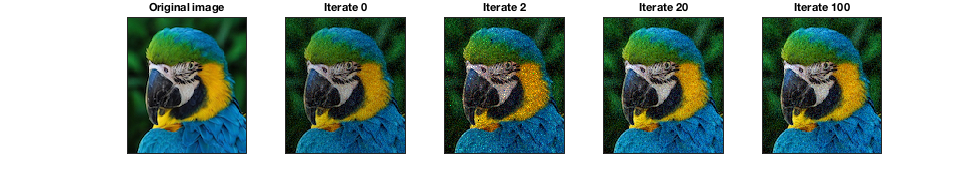
\includegraphics[scale=0.55]{parrot_signal_iterates} }
\hbox{\hspace{-2.5cm} 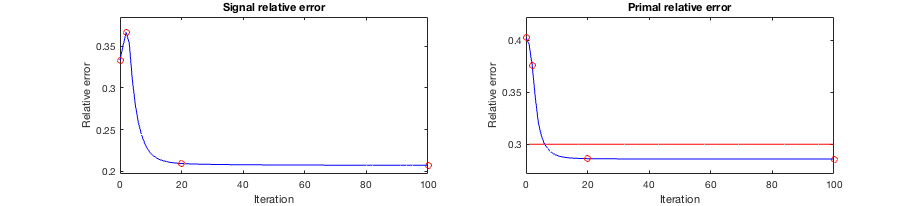
\includegraphics[scale=0.6]{parrot_signal_relative_error_2} }
\caption{Results from the first-order PLGD method (Algorithm \ref{Alg:PGD}) applied to a test image separated into its three RGB channels.  Left: signal relative error $||xx^*- \bar{x}\bar{x}^*||_F / ||\bar{x}\bar{x}^*||_F$.  Right: primal relative error $||\caA(xx^*)-b|| /  ||b||$ with red line indicating primal feasibility.  Red circles denote the iterate signals pictured above.  Original signal is $128 \times 128$ pixels, with an oversampling of $L = 8$ and noise ratio $\epsilon_\rel = 0.30$.  Measurements use the mean of the three color channel values.}
\label{Fig:parrot_signal_relative_error_2}
\end{figure}
% experiments.figure.noisyimage_signal_relerr_various_saga_iterates

Figure \ref{Fig:parrot_signal_relative_error_2} demonstrates the tendency of Algorithm \ref{Alg:PGD} to make significant progress during early iterates.  When the same set of models in Figure \ref{Fig:parrot_signal_relative_error_2} were solved with wflow, the red channel converged to an infeasible solution (with primal residual $0.300068$), the green channel converged to a feasible solution (with primal residual $0.288473$), and the blue channel diverged.  





Table \ref{Tab:relative_errors_saga_vs_wflow} and Figure \ref{Fig:parrot_signal_relative_error_2} highlight the effectiveness of the first-order PLGD method (Algorithm \ref{Alg:PGD}) for noisy phase retrieval problems.  
This method is typically is more robust than wflow (Algorithm \ref{Alg:wflow}) and tends to recover signals successfully when there is minimal oversampling. 
Among the phase retrieval models and methods considered in this chapter, the PLGD model (\ref{Eqn:PLGD_ch2}) is the best suited for large-scale, unstructured noisy phase retrieval problems.
In the next two chapters we present the theory behind the PLGD model and develop a first-order method (Algorithm \ref{Alg:PGD}) for optimizing this model.


